% Options for packages loaded elsewhere
\PassOptionsToPackage{unicode}{hyperref}
\PassOptionsToPackage{hyphens}{url}
%
\documentclass[
  english,
  man]{apa6}
\usepackage{lmodern}
\usepackage{amssymb,amsmath}
\usepackage{ifxetex,ifluatex}
\ifnum 0\ifxetex 1\fi\ifluatex 1\fi=0 % if pdftex
  \usepackage[T1]{fontenc}
  \usepackage[utf8]{inputenc}
  \usepackage{textcomp} % provide euro and other symbols
\else % if luatex or xetex
  \usepackage{unicode-math}
  \defaultfontfeatures{Scale=MatchLowercase}
  \defaultfontfeatures[\rmfamily]{Ligatures=TeX,Scale=1}
\fi
% Use upquote if available, for straight quotes in verbatim environments
\IfFileExists{upquote.sty}{\usepackage{upquote}}{}
\IfFileExists{microtype.sty}{% use microtype if available
  \usepackage[]{microtype}
  \UseMicrotypeSet[protrusion]{basicmath} % disable protrusion for tt fonts
}{}
\makeatletter
\@ifundefined{KOMAClassName}{% if non-KOMA class
  \IfFileExists{parskip.sty}{%
    \usepackage{parskip}
  }{% else
    \setlength{\parindent}{0pt}
    \setlength{\parskip}{6pt plus 2pt minus 1pt}}
}{% if KOMA class
  \KOMAoptions{parskip=half}}
\makeatother
\usepackage{xcolor}
\IfFileExists{xurl.sty}{\usepackage{xurl}}{} % add URL line breaks if available
\IfFileExists{bookmark.sty}{\usepackage{bookmark}}{\usepackage{hyperref}}
\hypersetup{
  pdftitle={Comparison of ICCs using IRT and CTT parameters},
  pdfauthor={Diego Figueiras1 \& John T. Kulas1},
  pdflang={en-EN},
  pdfkeywords={keywords},
  hidelinks,
  pdfcreator={LaTeX via pandoc}}
\urlstyle{same} % disable monospaced font for URLs
\usepackage{graphicx,grffile}
\makeatletter
\def\maxwidth{\ifdim\Gin@nat@width>\linewidth\linewidth\else\Gin@nat@width\fi}
\def\maxheight{\ifdim\Gin@nat@height>\textheight\textheight\else\Gin@nat@height\fi}
\makeatother
% Scale images if necessary, so that they will not overflow the page
% margins by default, and it is still possible to overwrite the defaults
% using explicit options in \includegraphics[width, height, ...]{}
\setkeys{Gin}{width=\maxwidth,height=\maxheight,keepaspectratio}
% Set default figure placement to htbp
\makeatletter
\def\fps@figure{htbp}
\makeatother
\setlength{\emergencystretch}{3em} % prevent overfull lines
\providecommand{\tightlist}{%
  \setlength{\itemsep}{0pt}\setlength{\parskip}{0pt}}
\setcounter{secnumdepth}{-\maxdimen} % remove section numbering
% Make \paragraph and \subparagraph free-standing
\ifx\paragraph\undefined\else
  \let\oldparagraph\paragraph
  \renewcommand{\paragraph}[1]{\oldparagraph{#1}\mbox{}}
\fi
\ifx\subparagraph\undefined\else
  \let\oldsubparagraph\subparagraph
  \renewcommand{\subparagraph}[1]{\oldsubparagraph{#1}\mbox{}}
\fi
% Manuscript styling
\usepackage{upgreek}
\captionsetup{font=singlespacing,justification=justified}

% Table formatting
\usepackage{longtable}
\usepackage{lscape}
% \usepackage[counterclockwise]{rotating}   % Landscape page setup for large tables
\usepackage{multirow}		% Table styling
\usepackage{tabularx}		% Control Column width
\usepackage[flushleft]{threeparttable}	% Allows for three part tables with a specified notes section
\usepackage{threeparttablex}            % Lets threeparttable work with longtable

% Create new environments so endfloat can handle them
% \newenvironment{ltable}
%   {\begin{landscape}\centering\begin{threeparttable}}
%   {\end{threeparttable}\end{landscape}}
\newenvironment{lltable}{\begin{landscape}\centering\begin{ThreePartTable}}{\end{ThreePartTable}\end{landscape}}

% Enables adjusting longtable caption width to table width
% Solution found at http://golatex.de/longtable-mit-caption-so-breit-wie-die-tabelle-t15767.html
\makeatletter
\newcommand\LastLTentrywidth{1em}
\newlength\longtablewidth
\setlength{\longtablewidth}{1in}
\newcommand{\getlongtablewidth}{\begingroup \ifcsname LT@\roman{LT@tables}\endcsname \global\longtablewidth=0pt \renewcommand{\LT@entry}[2]{\global\advance\longtablewidth by ##2\relax\gdef\LastLTentrywidth{##2}}\@nameuse{LT@\roman{LT@tables}} \fi \endgroup}

% \setlength{\parindent}{0.5in}
% \setlength{\parskip}{0pt plus 0pt minus 0pt}

% \usepackage{etoolbox}
\makeatletter
\patchcmd{\HyOrg@maketitle}
  {\section{\normalfont\normalsize\abstractname}}
  {\section*{\normalfont\normalsize\abstractname}}
  {}{\typeout{Failed to patch abstract.}}
\patchcmd{\HyOrg@maketitle}
  {\section{\protect\normalfont{\@title}}}
  {\section*{\protect\normalfont{\@title}}}
  {}{\typeout{Failed to patch title.}}
\makeatother
\shorttitle{Comparison of ICCs using IRT and CTT parameters}
\keywords{keywords\newline\indent Word count: X}
\DeclareDelayedFloatFlavor{ThreePartTable}{table}
\DeclareDelayedFloatFlavor{lltable}{table}
\DeclareDelayedFloatFlavor*{longtable}{table}
\makeatletter
\renewcommand{\efloat@iwrite}[1]{\immediate\expandafter\protected@write\csname efloat@post#1\endcsname{}}
\makeatother
\usepackage{lineno}

\linenumbers
\usepackage{csquotes}
\ifxetex
  % Load polyglossia as late as possible: uses bidi with RTL langages (e.g. Hebrew, Arabic)
  \usepackage{polyglossia}
  \setmainlanguage[]{english}
\else
  \usepackage[shorthands=off,main=english]{babel}
\fi

\title{Comparison of ICCs using IRT and CTT parameters}
\author{Diego Figueiras\textsuperscript{1} \& John T. Kulas\textsuperscript{1}}
\date{}


\authornote{

Add complete departmental affiliations for each author here. Each new line herein must be indented, like this line.

Enter author note here.

The authors made the following contributions. Diego Figueiras: Conceptualization, Writing - Original Draft Preparation, Writing - Review \& Editing; John T. Kulas: Writing - Review \& Editing.

Correspondence concerning this article should be addressed to Diego Figueiras, Postal address. E-mail: \href{mailto:figueirasd1@montclair.edu}{\nolinkurl{figueirasd1@montclair.edu}}

}

\affiliation{\vspace{0.5cm}\textsuperscript{1} Montclair State University}

\abstract{
One or two sentences providing a \textbf{basic introduction} to the field, comprehensible to a scientist in any discipline.

Two to three sentences of \textbf{more detailed background}, comprehensible to scientists in related disciplines.

One sentence clearly stating the \textbf{general problem} being addressed by this particular study.

One sentence summarizing the main result (with the words ``\textbf{here we show}'' or their equivalent).

Two or three sentences explaining what the \textbf{main result} reveals in direct comparison to what was thought to be the case previously, or how the main result adds to previous knowledge.

One or two sentences to put the results into a more \textbf{general context}.

Two or three sentences to provide a \textbf{broader perspective}, readily comprehensible to a scientist in any discipline.
}



\begin{document}
\maketitle

\hypertarget{introduction}{%
\section{Introduction}\label{introduction}}

Item characteristic curves are very often used by psychometricians to showcase and analyze the attributes of the item on a test or assessment. The x-axis shows a wide range of trait levels (ranging from high to low on the trait), while the y-axis displays probabilities of getting the item correct that range from 0 to 1. Each item has a curve. By looking at it, we can know the likelihood with which respondents of any trait level would answer any item correctly. If the curve is leaning towards the lower end of the trait level, this indicates that it is easy to answer the item correctly. On the contrary, if the curve is leaning towards the higher end of the trait level, this indicates that the item is difficult. If the curve is steep, this indicates high discrimination among respondents; if it is flat, it indicates no discrimination.

Psychometricians who examine ICCs usually do it using Item Response Theory and Rasch models to get the parameters necessary to plot the curves. In a 2PL model, these would be item difficulty and item discrimination. Item difficulty is the necessary trail level for a respondent to have a 50/50 chace to answer the item correctly. Item discrimination is the degree to which an item can differentiate among individuals with low and high levels of the trait. From a Classical Test Theory (CTT) frame of thinking, the difficulty of an item is determined by looking at the p-values of the items, while discrimination is determined by checking the Cronbach alpha and the corrected item total correlations. Psychometricians who look at these CTT parameters don't typically use them to plot ICCs.There is no reason for them not to, since ICCs based on CTT parameters could provide information as valuable as those based on IRT or Rasch without the need of being familiar with these models and with how to compute the necessary estimates. Fan states in summary that IRT and CTT \enquote{\ldots{} framework produce very similar item and person statistics} (p.379). Practitioners and researchers that don't use IRT or Rasch models and instead opt to follow a CTT philosophy would benefit from having ICCs that use CTT statistics. This study intends to show evidence of the overlapping nature of CTT and IRT parameters when it comes to plotting ICCs.

\hypertarget{methods}{%
\section{Methods}\label{methods}}

We used the formulas presented by Kulas, Smith, and Xu (2017).

Study 2 simulates a bunch of test data and then we generate ICCs based on the IRT model and then we compare that to our CTT estimates.
\#\# Participants

\hypertarget{material}{%
\subsection{Material}\label{material}}

\hypertarget{procedure}{%
\subsection{Procedure}\label{procedure}}

\hypertarget{data-analysis}{%
\subsection{Data analysis}\label{data-analysis}}

We used R (Version 4.0.3; R Core Team, 2020) and the R-packages \emph{dplyr} (Version 1.0.7; Wickham et al., 2021), \emph{DT} (Version 0.19; Xie, Cheng, \& Tan, 2021), \emph{forcats} (Version 0.5.1; Wickham, 2021a), \emph{formattable} (Version 0.2.1; Ren \& Russell, 2021), \emph{ggplot2} (Version 3.3.5; Wickham, 2016), \emph{jpeg} (Version 0.1.9; Urbanek, 2021), \emph{knitr} (Version 1.33; Xie, 2015), \emph{markdown} (Version 1.1; Allaire, Horner, Xie, Marti, \& Porte, 2019; Xie, Allaire, \& Grolemund, 2018; Xie, Dervieux, \& Riederer, 2020), \emph{officer} (Version 0.3.19; Gohel, 2021), \emph{papaja} (Version 0.1.0.9997; Aust \& Barth, 2020), \emph{pdftools} (Version 3.0.1; Ooms, 2021), \emph{psych} (Version 2.1.6; Revelle, 2021), \emph{purrr} (Version 0.3.4; Henry \& Wickham, 2020), \emph{readr} (Version 2.0.1; Wickham \& Hester, 2021), \emph{readxl} (Version 1.3.1; Wickham \& Bryan, 2019), \emph{reticulate} (Version 1.20; Ushey, Allaire, \& Tang, 2021), \emph{rmarkdown} (Version 2.10; Xie et al., 2018, 2020), \emph{shiny} (Version 1.6.0; Chang et al., 2021), \emph{stringr} (Version 1.4.0; Wickham, 2019), \emph{tibble} (Version 3.1.4; Müller \& Wickham, 2021), \emph{tidyr} (Version 1.1.3; Wickham, 2021b), \emph{tidyverse} (Version 1.3.1; Wickham, Averick, et al., 2019), and \emph{tinytex} (Version 0.33; Xie, 2019) for all our analyses.

\begin{figure}
\centering
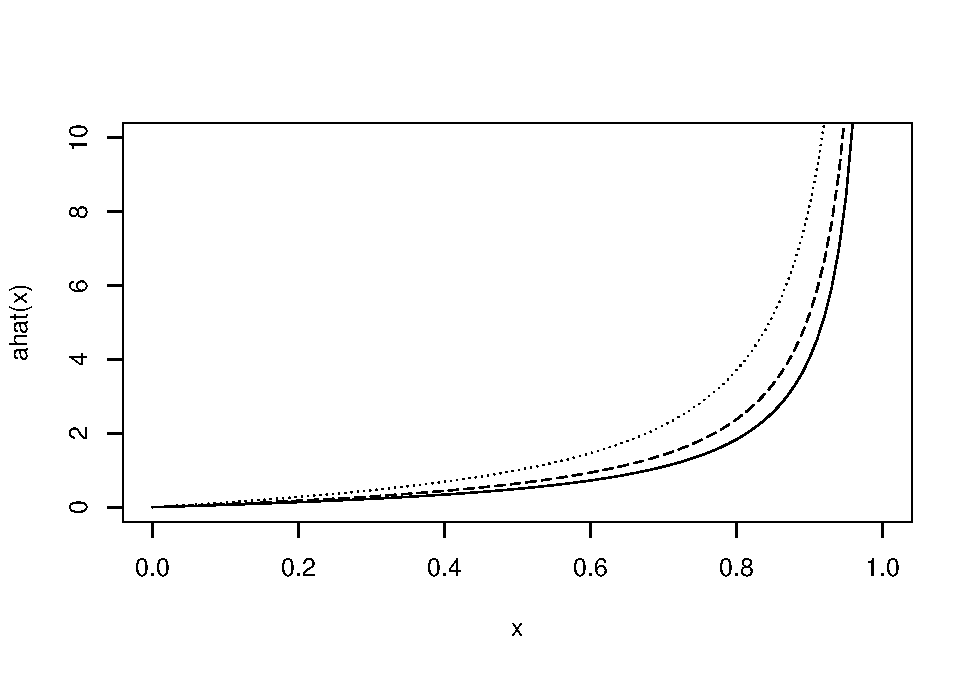
\includegraphics{ICC_project_files/figure-latex/unnamed-chunk-2-1.pdf}
\caption{\label{fig:unnamed-chunk-2}Relationship between IRT a parameter and CTT corrected-item total correlations.}
\end{figure}

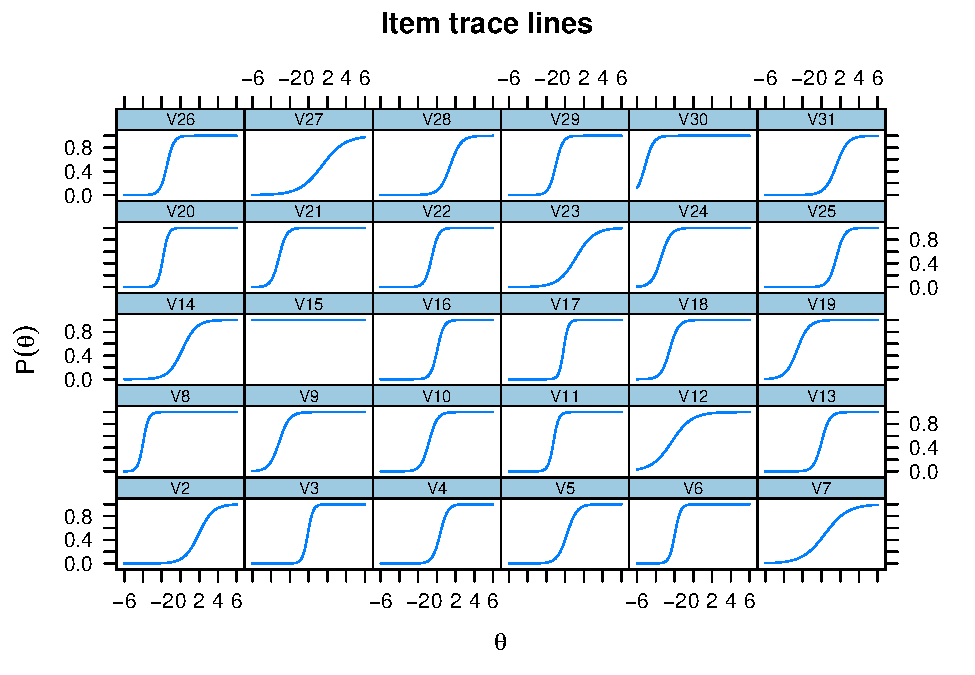
\includegraphics{ICC_project_files/figure-latex/unnamed-chunk-3-1.pdf}

\begin{verbatim}
## Iteration: 1, Log-Lik: -98116.710, Max-Change: 4.09843Iteration: 2, Log-Lik: -93555.376, Max-Change: 2.36211Iteration: 3, Log-Lik: -92095.297, Max-Change: 0.86232Iteration: 4, Log-Lik: -91400.840, Max-Change: 0.57759Iteration: 5, Log-Lik: -90976.438, Max-Change: 0.53628Iteration: 6, Log-Lik: -90733.642, Max-Change: 0.43949Iteration: 7, Log-Lik: -90530.551, Max-Change: 0.28402Iteration: 8, Log-Lik: -90398.548, Max-Change: 0.35077Iteration: 9, Log-Lik: -90294.315, Max-Change: 0.36077Iteration: 10, Log-Lik: -90233.325, Max-Change: 0.24911Iteration: 11, Log-Lik: -90186.125, Max-Change: 0.24444Iteration: 12, Log-Lik: -90154.098, Max-Change: 0.18850Iteration: 13, Log-Lik: -90129.582, Max-Change: 0.17557Iteration: 14, Log-Lik: -90112.262, Max-Change: 0.14661Iteration: 15, Log-Lik: -90098.850, Max-Change: 0.14473Iteration: 16, Log-Lik: -90088.026, Max-Change: 0.10233Iteration: 17, Log-Lik: -90080.549, Max-Change: 0.12783Iteration: 18, Log-Lik: -90074.739, Max-Change: 0.09322Iteration: 19, Log-Lik: -90070.174, Max-Change: 0.10813Iteration: 20, Log-Lik: -90066.817, Max-Change: 0.08788Iteration: 21, Log-Lik: -90064.371, Max-Change: 0.08676Iteration: 22, Log-Lik: -90062.457, Max-Change: 0.10631Iteration: 23, Log-Lik: -90060.862, Max-Change: 0.07361Iteration: 24, Log-Lik: -90059.658, Max-Change: 0.11716Iteration: 25, Log-Lik: -90058.414, Max-Change: 0.05900Iteration: 26, Log-Lik: -90057.565, Max-Change: 0.63640Iteration: 27, Log-Lik: -90056.122, Max-Change: 0.14655Iteration: 28, Log-Lik: -90055.809, Max-Change: 0.91866Iteration: 29, Log-Lik: -90055.074, Max-Change: 0.14450Iteration: 30, Log-Lik: -90054.358, Max-Change: 0.15677Iteration: 31, Log-Lik: -90053.967, Max-Change: 0.35165Iteration: 32, Log-Lik: -90053.643, Max-Change: 0.00585Iteration: 33, Log-Lik: -90053.449, Max-Change: 0.00453Iteration: 34, Log-Lik: -90053.016, Max-Change: 0.00352Iteration: 35, Log-Lik: -90052.919, Max-Change: 0.00258Iteration: 36, Log-Lik: -90052.850, Max-Change: 0.00312Iteration: 37, Log-Lik: -90052.563, Max-Change: 0.00161Iteration: 38, Log-Lik: -90052.537, Max-Change: 0.00534Iteration: 39, Log-Lik: -90052.518, Max-Change: 0.00203Iteration: 40, Log-Lik: -90052.508, Max-Change: 0.00187Iteration: 41, Log-Lik: -90052.490, Max-Change: 0.00118Iteration: 42, Log-Lik: -90052.483, Max-Change: 0.00092Iteration: 43, Log-Lik: -90052.462, Max-Change: 0.00120Iteration: 44, Log-Lik: -90052.451, Max-Change: 0.00083Iteration: 45, Log-Lik: -90052.445, Max-Change: 0.00084Iteration: 46, Log-Lik: -90052.423, Max-Change: 0.00069Iteration: 47, Log-Lik: -90052.421, Max-Change: 0.00072Iteration: 48, Log-Lik: -90052.419, Max-Change: 0.00023Iteration: 49, Log-Lik: -90052.419, Max-Change: 0.00019Iteration: 50, Log-Lik: -90052.418, Max-Change: 0.00047Iteration: 51, Log-Lik: -90052.417, Max-Change: 0.00059Iteration: 52, Log-Lik: -90052.416, Max-Change: 0.00038Iteration: 53, Log-Lik: -90052.415, Max-Change: 0.00061Iteration: 54, Log-Lik: -90052.414, Max-Change: 0.00026Iteration: 55, Log-Lik: -90052.414, Max-Change: 0.00021Iteration: 56, Log-Lik: -90052.414, Max-Change: 0.00035Iteration: 57, Log-Lik: -90052.413, Max-Change: 0.00018Iteration: 58, Log-Lik: -90052.413, Max-Change: 0.00074Iteration: 59, Log-Lik: -90052.413, Max-Change: 0.00034Iteration: 60, Log-Lik: -90052.412, Max-Change: 0.00048Iteration: 61, Log-Lik: -90052.412, Max-Change: 0.00043Iteration: 62, Log-Lik: -90052.411, Max-Change: 0.00068Iteration: 63, Log-Lik: -90052.411, Max-Change: 0.00031Iteration: 64, Log-Lik: -90052.411, Max-Change: 0.00025Iteration: 65, Log-Lik: -90052.410, Max-Change: 0.00035Iteration: 66, Log-Lik: -90052.410, Max-Change: 0.00020Iteration: 67, Log-Lik: -90052.410, Max-Change: 0.00016Iteration: 68, Log-Lik: -90052.410, Max-Change: 0.00031Iteration: 69, Log-Lik: -90052.409, Max-Change: 0.00056Iteration: 70, Log-Lik: -90052.409, Max-Change: 0.00029Iteration: 71, Log-Lik: -90052.409, Max-Change: 0.00046Iteration: 72, Log-Lik: -90052.408, Max-Change: 0.00021Iteration: 73, Log-Lik: -90052.408, Max-Change: 0.00017Iteration: 74, Log-Lik: -90052.408, Max-Change: 0.00030Iteration: 75, Log-Lik: -90052.408, Max-Change: 0.00014Iteration: 76, Log-Lik: -90052.408, Max-Change: 0.00055Iteration: 77, Log-Lik: -90052.407, Max-Change: 0.00026Iteration: 78, Log-Lik: -90052.407, Max-Change: 0.00039Iteration: 79, Log-Lik: -90052.407, Max-Change: 0.00033Iteration: 80, Log-Lik: -90052.407, Max-Change: 0.00052Iteration: 81, Log-Lik: -90052.406, Max-Change: 0.00025Iteration: 82, Log-Lik: -90052.406, Max-Change: 0.00019Iteration: 83, Log-Lik: -90052.406, Max-Change: 0.00030Iteration: 84, Log-Lik: -90052.406, Max-Change: 0.00015Iteration: 85, Log-Lik: -90052.406, Max-Change: 0.00012Iteration: 86, Log-Lik: -90052.406, Max-Change: 0.00030Iteration: 87, Log-Lik: -90052.405, Max-Change: 0.00044Iteration: 88, Log-Lik: -90052.405, Max-Change: 0.00023Iteration: 89, Log-Lik: -90052.405, Max-Change: 0.00036Iteration: 90, Log-Lik: -90052.405, Max-Change: 0.00017Iteration: 91, Log-Lik: -90052.405, Max-Change: 0.00014Iteration: 92, Log-Lik: -90052.405, Max-Change: 0.00031Iteration: 93, Log-Lik: -90052.404, Max-Change: 0.00053Iteration: 94, Log-Lik: -90052.404, Max-Change: 0.00023Iteration: 95, Log-Lik: -90052.404, Max-Change: 0.00035Iteration: 96, Log-Lik: -90052.404, Max-Change: 0.00018Iteration: 97, Log-Lik: -90052.404, Max-Change: 0.00014Iteration: 98, Log-Lik: -90052.404, Max-Change: 0.00031Iteration: 99, Log-Lik: -90052.404, Max-Change: 0.00010Iteration: 100, Log-Lik: -90052.404, Max-Change: 0.00042Iteration: 101, Log-Lik: -90052.403, Max-Change: 0.00021Iteration: 102, Log-Lik: -90052.403, Max-Change: 0.00033Iteration: 103, Log-Lik: -90052.403, Max-Change: 0.00026Iteration: 104, Log-Lik: -90052.403, Max-Change: 0.00040Iteration: 105, Log-Lik: -90052.403, Max-Change: 0.00020Iteration: 106, Log-Lik: -90052.403, Max-Change: 0.00016Iteration: 107, Log-Lik: -90052.403, Max-Change: 0.00032Iteration: 108, Log-Lik: -90052.402, Max-Change: 0.00012Iteration: 109, Log-Lik: -90052.402, Max-Change: 0.00047Iteration: 110, Log-Lik: -90052.402, Max-Change: 0.00023Iteration: 111, Log-Lik: -90052.402, Max-Change: 0.00037Iteration: 112, Log-Lik: -90052.402, Max-Change: 0.00031Iteration: 113, Log-Lik: -90052.402, Max-Change: 0.00010
## 
## Calculating information matrix...
\end{verbatim}

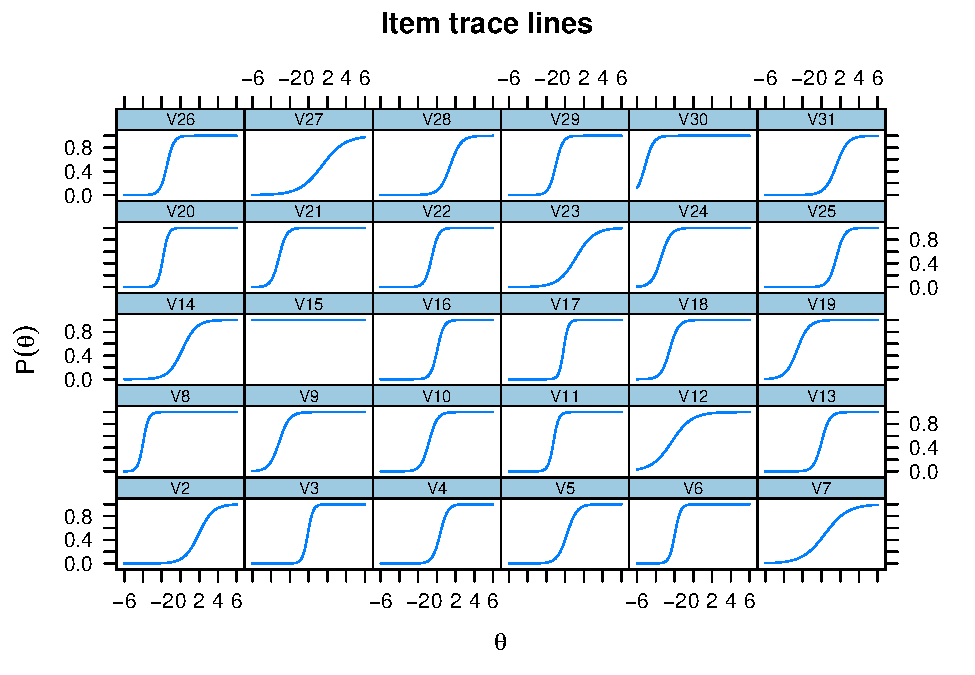
\includegraphics{ICC_project_files/figure-latex/unnamed-chunk-4-1.pdf}

\begin{verbatim}
## Iteration: 1, Log-Lik: -98116.710, Max-Change: 4.09843Iteration: 2, Log-Lik: -93555.376, Max-Change: 2.36211Iteration: 3, Log-Lik: -92095.297, Max-Change: 0.86232Iteration: 4, Log-Lik: -91400.840, Max-Change: 0.57759Iteration: 5, Log-Lik: -90976.438, Max-Change: 0.53628Iteration: 6, Log-Lik: -90733.642, Max-Change: 0.43949Iteration: 7, Log-Lik: -90530.551, Max-Change: 0.28402Iteration: 8, Log-Lik: -90398.548, Max-Change: 0.35077Iteration: 9, Log-Lik: -90294.315, Max-Change: 0.36077Iteration: 10, Log-Lik: -90233.325, Max-Change: 0.24911Iteration: 11, Log-Lik: -90186.125, Max-Change: 0.24444Iteration: 12, Log-Lik: -90154.098, Max-Change: 0.18850Iteration: 13, Log-Lik: -90129.582, Max-Change: 0.17557Iteration: 14, Log-Lik: -90112.262, Max-Change: 0.14661Iteration: 15, Log-Lik: -90098.850, Max-Change: 0.14473Iteration: 16, Log-Lik: -90088.026, Max-Change: 0.10233Iteration: 17, Log-Lik: -90080.549, Max-Change: 0.12783Iteration: 18, Log-Lik: -90074.739, Max-Change: 0.09322Iteration: 19, Log-Lik: -90070.174, Max-Change: 0.10813Iteration: 20, Log-Lik: -90066.817, Max-Change: 0.08788Iteration: 21, Log-Lik: -90064.371, Max-Change: 0.08676Iteration: 22, Log-Lik: -90062.457, Max-Change: 0.10631Iteration: 23, Log-Lik: -90060.862, Max-Change: 0.07361Iteration: 24, Log-Lik: -90059.658, Max-Change: 0.11716Iteration: 25, Log-Lik: -90058.414, Max-Change: 0.05900Iteration: 26, Log-Lik: -90057.565, Max-Change: 0.63640Iteration: 27, Log-Lik: -90056.122, Max-Change: 0.14655Iteration: 28, Log-Lik: -90055.809, Max-Change: 0.91866Iteration: 29, Log-Lik: -90055.074, Max-Change: 0.14450Iteration: 30, Log-Lik: -90054.358, Max-Change: 0.15677Iteration: 31, Log-Lik: -90053.967, Max-Change: 0.35165Iteration: 32, Log-Lik: -90053.643, Max-Change: 0.00585Iteration: 33, Log-Lik: -90053.449, Max-Change: 0.00453Iteration: 34, Log-Lik: -90053.016, Max-Change: 0.00352Iteration: 35, Log-Lik: -90052.919, Max-Change: 0.00258Iteration: 36, Log-Lik: -90052.850, Max-Change: 0.00312Iteration: 37, Log-Lik: -90052.563, Max-Change: 0.00161Iteration: 38, Log-Lik: -90052.537, Max-Change: 0.00534Iteration: 39, Log-Lik: -90052.518, Max-Change: 0.00203Iteration: 40, Log-Lik: -90052.508, Max-Change: 0.00187Iteration: 41, Log-Lik: -90052.490, Max-Change: 0.00118Iteration: 42, Log-Lik: -90052.483, Max-Change: 0.00092Iteration: 43, Log-Lik: -90052.462, Max-Change: 0.00120Iteration: 44, Log-Lik: -90052.451, Max-Change: 0.00083Iteration: 45, Log-Lik: -90052.445, Max-Change: 0.00084Iteration: 46, Log-Lik: -90052.423, Max-Change: 0.00069Iteration: 47, Log-Lik: -90052.421, Max-Change: 0.00072Iteration: 48, Log-Lik: -90052.419, Max-Change: 0.00023Iteration: 49, Log-Lik: -90052.419, Max-Change: 0.00019Iteration: 50, Log-Lik: -90052.418, Max-Change: 0.00047Iteration: 51, Log-Lik: -90052.417, Max-Change: 0.00059Iteration: 52, Log-Lik: -90052.416, Max-Change: 0.00038Iteration: 53, Log-Lik: -90052.415, Max-Change: 0.00061Iteration: 54, Log-Lik: -90052.414, Max-Change: 0.00026Iteration: 55, Log-Lik: -90052.414, Max-Change: 0.00021Iteration: 56, Log-Lik: -90052.414, Max-Change: 0.00035Iteration: 57, Log-Lik: -90052.413, Max-Change: 0.00018Iteration: 58, Log-Lik: -90052.413, Max-Change: 0.00074Iteration: 59, Log-Lik: -90052.413, Max-Change: 0.00034Iteration: 60, Log-Lik: -90052.412, Max-Change: 0.00048Iteration: 61, Log-Lik: -90052.412, Max-Change: 0.00043Iteration: 62, Log-Lik: -90052.411, Max-Change: 0.00068Iteration: 63, Log-Lik: -90052.411, Max-Change: 0.00031Iteration: 64, Log-Lik: -90052.411, Max-Change: 0.00025Iteration: 65, Log-Lik: -90052.410, Max-Change: 0.00035Iteration: 66, Log-Lik: -90052.410, Max-Change: 0.00020Iteration: 67, Log-Lik: -90052.410, Max-Change: 0.00016Iteration: 68, Log-Lik: -90052.410, Max-Change: 0.00031Iteration: 69, Log-Lik: -90052.409, Max-Change: 0.00056Iteration: 70, Log-Lik: -90052.409, Max-Change: 0.00029Iteration: 71, Log-Lik: -90052.409, Max-Change: 0.00046Iteration: 72, Log-Lik: -90052.408, Max-Change: 0.00021Iteration: 73, Log-Lik: -90052.408, Max-Change: 0.00017Iteration: 74, Log-Lik: -90052.408, Max-Change: 0.00030Iteration: 75, Log-Lik: -90052.408, Max-Change: 0.00014Iteration: 76, Log-Lik: -90052.408, Max-Change: 0.00055Iteration: 77, Log-Lik: -90052.407, Max-Change: 0.00026Iteration: 78, Log-Lik: -90052.407, Max-Change: 0.00039Iteration: 79, Log-Lik: -90052.407, Max-Change: 0.00033Iteration: 80, Log-Lik: -90052.407, Max-Change: 0.00052Iteration: 81, Log-Lik: -90052.406, Max-Change: 0.00025Iteration: 82, Log-Lik: -90052.406, Max-Change: 0.00019Iteration: 83, Log-Lik: -90052.406, Max-Change: 0.00030Iteration: 84, Log-Lik: -90052.406, Max-Change: 0.00015Iteration: 85, Log-Lik: -90052.406, Max-Change: 0.00012Iteration: 86, Log-Lik: -90052.406, Max-Change: 0.00030Iteration: 87, Log-Lik: -90052.405, Max-Change: 0.00044Iteration: 88, Log-Lik: -90052.405, Max-Change: 0.00023Iteration: 89, Log-Lik: -90052.405, Max-Change: 0.00036Iteration: 90, Log-Lik: -90052.405, Max-Change: 0.00017Iteration: 91, Log-Lik: -90052.405, Max-Change: 0.00014Iteration: 92, Log-Lik: -90052.405, Max-Change: 0.00031Iteration: 93, Log-Lik: -90052.404, Max-Change: 0.00053Iteration: 94, Log-Lik: -90052.404, Max-Change: 0.00023Iteration: 95, Log-Lik: -90052.404, Max-Change: 0.00035Iteration: 96, Log-Lik: -90052.404, Max-Change: 0.00018Iteration: 97, Log-Lik: -90052.404, Max-Change: 0.00014Iteration: 98, Log-Lik: -90052.404, Max-Change: 0.00031Iteration: 99, Log-Lik: -90052.404, Max-Change: 0.00010Iteration: 100, Log-Lik: -90052.404, Max-Change: 0.00042Iteration: 101, Log-Lik: -90052.403, Max-Change: 0.00021Iteration: 102, Log-Lik: -90052.403, Max-Change: 0.00033Iteration: 103, Log-Lik: -90052.403, Max-Change: 0.00026Iteration: 104, Log-Lik: -90052.403, Max-Change: 0.00040Iteration: 105, Log-Lik: -90052.403, Max-Change: 0.00020Iteration: 106, Log-Lik: -90052.403, Max-Change: 0.00016Iteration: 107, Log-Lik: -90052.403, Max-Change: 0.00032Iteration: 108, Log-Lik: -90052.402, Max-Change: 0.00012Iteration: 109, Log-Lik: -90052.402, Max-Change: 0.00047Iteration: 110, Log-Lik: -90052.402, Max-Change: 0.00023Iteration: 111, Log-Lik: -90052.402, Max-Change: 0.00037Iteration: 112, Log-Lik: -90052.402, Max-Change: 0.00031Iteration: 113, Log-Lik: -90052.402, Max-Change: 0.00010
\end{verbatim}

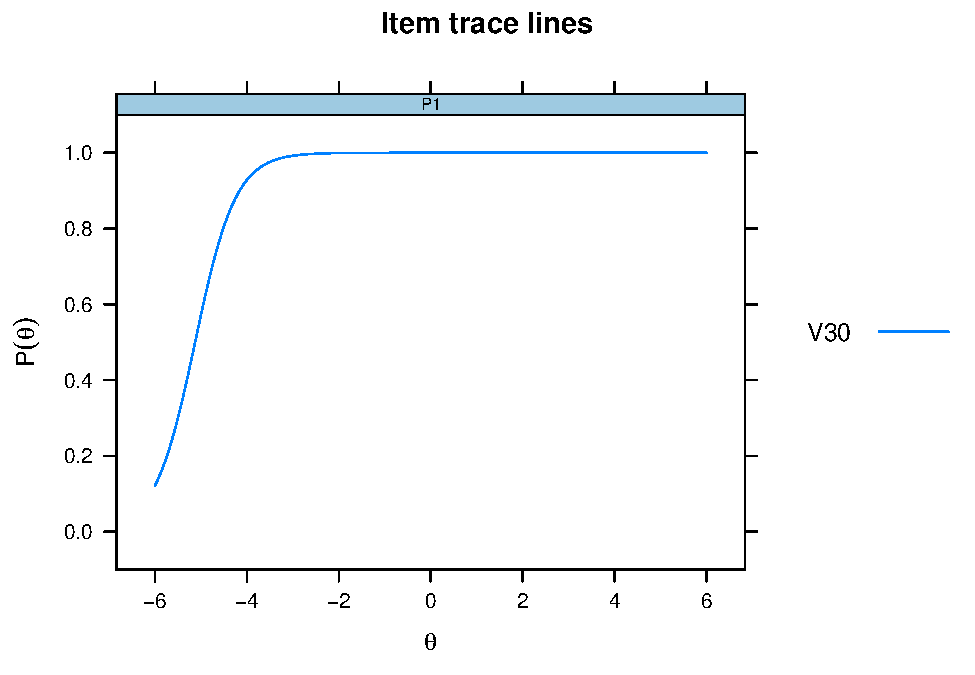
\includegraphics{ICC_project_files/figure-latex/unnamed-chunk-4-2.pdf}

\begin{verbatim}
## Warning in mean.default(data$v10): argument is not numeric or logical: returning
## NA
\end{verbatim}

\begin{verbatim}
## Warning in alpha(data): Some items were negatively correlated with the total scale and probably 
## should be reversed.  
## To do this, run the function again with the 'check.keys=TRUE' option
\end{verbatim}

\begin{verbatim}
## Some items ( V15 ) were negatively correlated with the total scale and 
## probably should be reversed.  
## To do this, run the function again with the 'check.keys=TRUE' option
\end{verbatim}

\begin{verbatim}
## 
## Reliability analysis   
## Call: alpha(x = data)
## 
##   raw_alpha std.alpha G6(smc) average_r S/N    ase mean   sd median_r
##       0.88      0.86    0.87      0.17 6.2 0.0015 0.65 0.17     0.15
## 
##  lower alpha upper     95% confidence boundaries
## 0.88 0.88 0.89 
## 
##  Reliability if an item is dropped:
##     raw_alpha std.alpha G6(smc) average_r S/N alpha se var.r med.r
## V2       0.88      0.86    0.87      0.17 6.1   0.0015 0.020  0.16
## V3       0.87      0.85    0.86      0.16 5.7   0.0016 0.017  0.15
## V4       0.87      0.85    0.86      0.17 5.8   0.0016 0.018  0.15
## V5       0.88      0.85    0.87      0.17 5.8   0.0015 0.018  0.15
## V6       0.88      0.86    0.87      0.17 6.0   0.0015 0.019  0.15
## V7       0.88      0.86    0.87      0.17 6.1   0.0014 0.020  0.16
## V8       0.88      0.87    0.88      0.18 6.4   0.0015 0.018  0.17
## V9       0.88      0.86    0.87      0.18 6.2   0.0015 0.020  0.16
## V10      0.88      0.85    0.86      0.17 5.8   0.0015 0.018  0.15
## V11      0.88      0.85    0.86      0.17 5.8   0.0015 0.018  0.15
## V12      0.88      0.86    0.87      0.17 6.1   0.0015 0.020  0.16
## V13      0.87      0.85    0.86      0.17 5.8   0.0016 0.018  0.15
## V14      0.88      0.86    0.87      0.17 5.9   0.0015 0.019  0.15
## V15      0.88      0.87    0.88      0.18 6.5   0.0015 0.018  0.17
## V16      0.87      0.85    0.86      0.16 5.7   0.0016 0.017  0.15
## V17      0.87      0.85    0.86      0.16 5.6   0.0016 0.017  0.15
## V18      0.88      0.86    0.87      0.17 6.1   0.0015 0.020  0.16
## V19      0.88      0.86    0.87      0.17 6.1   0.0015 0.020  0.16
## V20      0.88      0.86    0.87      0.17 5.9   0.0015 0.019  0.15
## V21      0.88      0.86    0.87      0.18 6.3   0.0015 0.019  0.16
## V22      0.87      0.85    0.86      0.16 5.7   0.0016 0.018  0.15
## V23      0.88      0.86    0.87      0.17 6.1   0.0015 0.020  0.15
## V24      0.88      0.86    0.87      0.18 6.3   0.0015 0.019  0.16
## V25      0.88      0.86    0.87      0.17 6.1   0.0015 0.019  0.15
## V26      0.88      0.85    0.87      0.17 5.8   0.0015 0.019  0.15
## V27      0.88      0.86    0.87      0.17 6.1   0.0014 0.020  0.16
## V28      0.88      0.86    0.87      0.17 6.0   0.0015 0.019  0.15
## V29      0.88      0.85    0.86      0.17 5.8   0.0015 0.018  0.15
## V30      0.88      0.87    0.88      0.18 6.5   0.0015 0.018  0.17
## V31      0.88      0.86    0.87      0.17 6.1   0.0015 0.019  0.15
## 
##  Item statistics 
##         n  raw.r std.r   r.cor  r.drop mean    sd
## V2  10000  0.366  0.36  0.3121  0.3092 0.12 0.325
## V3  10000  0.748  0.70  0.7108  0.6999 0.53 0.499
## V4  10000  0.665  0.62  0.6141  0.6074 0.39 0.488
## V5  10000  0.629  0.58  0.5730  0.5656 0.44 0.496
## V6  10000  0.395  0.47  0.4512  0.3613 0.96 0.203
## V7  10000  0.422  0.39  0.3453  0.3386 0.43 0.495
## V8  10000  0.041  0.13  0.0656  0.0383 1.00 0.014
## V9  10000  0.198  0.28  0.2306  0.1762 0.99 0.115
## V10 10000  0.627  0.61  0.6077  0.5717 0.74 0.436
## V11 10000  0.590  0.62  0.6151  0.5437 0.86 0.343
## V12 10000  0.341  0.35  0.3060  0.2802 0.86 0.343
## V13 10000  0.681  0.63  0.6307  0.6235 0.49 0.500
## V14 10000  0.545  0.51  0.4800  0.4718 0.45 0.498
## V15 10000 -0.003  0.07 -0.0044 -0.0049 1.00 0.010
## V16 10000  0.716  0.67  0.6708  0.6633 0.48 0.500
## V17 10000  0.763  0.71  0.7286  0.7179 0.56 0.497
## V18 10000  0.291  0.36  0.3174  0.2612 0.97 0.164
## V19 10000  0.303  0.36  0.3100  0.2668 0.96 0.201
## V20 10000  0.419  0.49  0.4751  0.3838 0.95 0.216
## V21 10000  0.160  0.25  0.1894  0.1450 0.99 0.077
## V22 10000  0.691  0.67  0.6672  0.6386 0.68 0.468
## V23 10000  0.434  0.41  0.3677  0.3608 0.27 0.443
## V24 10000  0.154  0.24  0.1777  0.1384 0.99 0.083
## V25 10000  0.431  0.42  0.3818  0.3810 0.10 0.306
## V26 10000  0.529  0.56  0.5525  0.4825 0.89 0.318
## V27 10000  0.375  0.35  0.3054  0.2985 0.26 0.438
## V28 10000  0.457  0.44  0.4022  0.3987 0.16 0.362
## V29 10000  0.622  0.62  0.6200  0.5709 0.80 0.403
## V30 10000  0.024  0.10  0.0314  0.0223 1.00 0.010
## V31 10000  0.430  0.41  0.3762  0.3733 0.14 0.345
## 
## Non missing response frequency for each item
##        0    1 miss
## V2  0.88 0.12    0
## V3  0.47 0.53    0
## V4  0.61 0.39    0
## V5  0.56 0.44    0
## V6  0.04 0.96    0
## V7  0.57 0.43    0
## V8  0.00 1.00    0
## V9  0.01 0.99    0
## V10 0.26 0.74    0
## V11 0.14 0.86    0
## V12 0.14 0.86    0
## V13 0.51 0.49    0
## V14 0.55 0.45    0
## V15 0.00 1.00    0
## V16 0.52 0.48    0
## V17 0.44 0.56    0
## V18 0.03 0.97    0
## V19 0.04 0.96    0
## V20 0.05 0.95    0
## V21 0.01 0.99    0
## V22 0.32 0.68    0
## V23 0.73 0.27    0
## V24 0.01 0.99    0
## V25 0.90 0.10    0
## V26 0.11 0.89    0
## V27 0.74 0.26    0
## V28 0.84 0.16    0
## V29 0.20 0.80    0
## V30 0.00 1.00    0
## V31 0.86 0.14    0
\end{verbatim}

\begin{verbatim}
## Warning: package 'gridExtra' was built under R version 4.0.5
\end{verbatim}

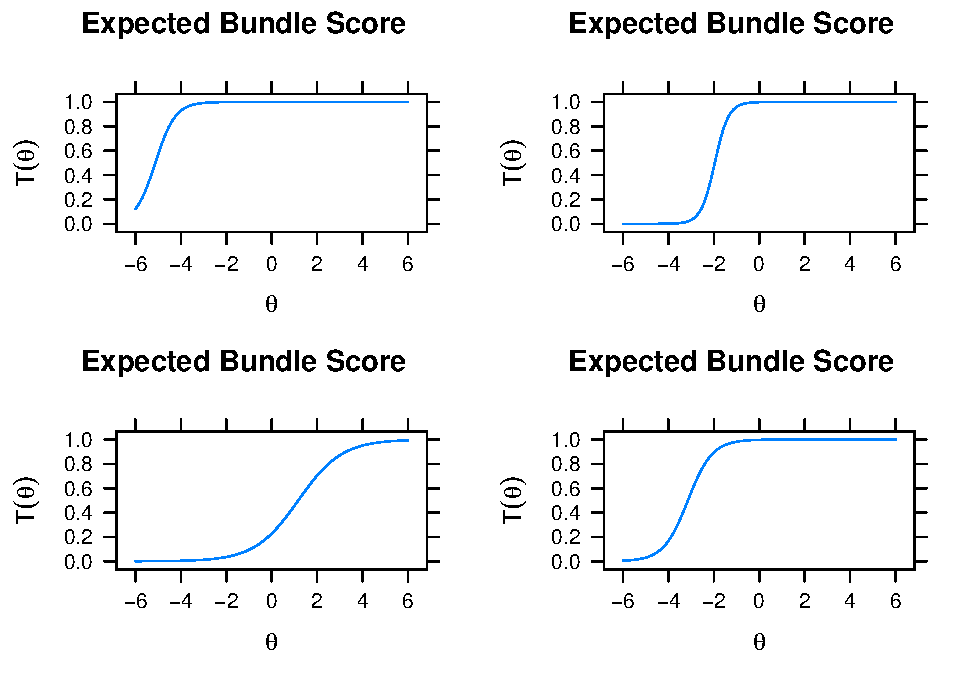
\includegraphics{ICC_project_files/figure-latex/unnamed-chunk-4-3.pdf}

\begin{verbatim}
## Warning in mean.default(data$i28): argument is not numeric or logical: returning
## NA
\end{verbatim}

\begin{verbatim}
## Warning in alpha(data): Some items were negatively correlated with the total scale and probably 
## should be reversed.  
## To do this, run the function again with the 'check.keys=TRUE' option
\end{verbatim}

\begin{verbatim}
## Some items ( V15 ) were negatively correlated with the total scale and 
## probably should be reversed.  
## To do this, run the function again with the 'check.keys=TRUE' option
\end{verbatim}

\begin{verbatim}
## 
## Reliability analysis   
## Call: alpha(x = data)
## 
##   raw_alpha std.alpha G6(smc) average_r S/N    ase mean   sd median_r
##       0.88      0.86    0.87      0.17 6.2 0.0015 0.65 0.17     0.15
## 
##  lower alpha upper     95% confidence boundaries
## 0.88 0.88 0.89 
## 
##  Reliability if an item is dropped:
##     raw_alpha std.alpha G6(smc) average_r S/N alpha se var.r med.r
## V2       0.88      0.86    0.87      0.17 6.1   0.0015 0.020  0.16
## V3       0.87      0.85    0.86      0.16 5.7   0.0016 0.017  0.15
## V4       0.87      0.85    0.86      0.17 5.8   0.0016 0.018  0.15
## V5       0.88      0.85    0.87      0.17 5.8   0.0015 0.018  0.15
## V6       0.88      0.86    0.87      0.17 6.0   0.0015 0.019  0.15
## V7       0.88      0.86    0.87      0.17 6.1   0.0014 0.020  0.16
## V8       0.88      0.87    0.88      0.18 6.4   0.0015 0.018  0.17
## V9       0.88      0.86    0.87      0.18 6.2   0.0015 0.020  0.16
## V10      0.88      0.85    0.86      0.17 5.8   0.0015 0.018  0.15
## V11      0.88      0.85    0.86      0.17 5.8   0.0015 0.018  0.15
## V12      0.88      0.86    0.87      0.17 6.1   0.0015 0.020  0.16
## V13      0.87      0.85    0.86      0.17 5.8   0.0016 0.018  0.15
## V14      0.88      0.86    0.87      0.17 5.9   0.0015 0.019  0.15
## V15      0.88      0.87    0.88      0.18 6.5   0.0015 0.018  0.17
## V16      0.87      0.85    0.86      0.16 5.7   0.0016 0.017  0.15
## V17      0.87      0.85    0.86      0.16 5.6   0.0016 0.017  0.15
## V18      0.88      0.86    0.87      0.17 6.1   0.0015 0.020  0.16
## V19      0.88      0.86    0.87      0.17 6.1   0.0015 0.020  0.16
## V20      0.88      0.86    0.87      0.17 5.9   0.0015 0.019  0.15
## V21      0.88      0.86    0.87      0.18 6.3   0.0015 0.019  0.16
## V22      0.87      0.85    0.86      0.16 5.7   0.0016 0.018  0.15
## V23      0.88      0.86    0.87      0.17 6.1   0.0015 0.020  0.15
## V24      0.88      0.86    0.87      0.18 6.3   0.0015 0.019  0.16
## V25      0.88      0.86    0.87      0.17 6.1   0.0015 0.019  0.15
## V26      0.88      0.85    0.87      0.17 5.8   0.0015 0.019  0.15
## V27      0.88      0.86    0.87      0.17 6.1   0.0014 0.020  0.16
## V28      0.88      0.86    0.87      0.17 6.0   0.0015 0.019  0.15
## V29      0.88      0.85    0.86      0.17 5.8   0.0015 0.018  0.15
## V30      0.88      0.87    0.88      0.18 6.5   0.0015 0.018  0.17
## V31      0.88      0.86    0.87      0.17 6.1   0.0015 0.019  0.15
## 
##  Item statistics 
##         n  raw.r std.r   r.cor  r.drop mean    sd
## V2  10000  0.366  0.36  0.3121  0.3092 0.12 0.325
## V3  10000  0.748  0.70  0.7108  0.6999 0.53 0.499
## V4  10000  0.665  0.62  0.6141  0.6074 0.39 0.488
## V5  10000  0.629  0.58  0.5730  0.5656 0.44 0.496
## V6  10000  0.395  0.47  0.4512  0.3613 0.96 0.203
## V7  10000  0.422  0.39  0.3453  0.3386 0.43 0.495
## V8  10000  0.041  0.13  0.0656  0.0383 1.00 0.014
## V9  10000  0.198  0.28  0.2306  0.1762 0.99 0.115
## V10 10000  0.627  0.61  0.6077  0.5717 0.74 0.436
## V11 10000  0.590  0.62  0.6151  0.5437 0.86 0.343
## V12 10000  0.341  0.35  0.3060  0.2802 0.86 0.343
## V13 10000  0.681  0.63  0.6307  0.6235 0.49 0.500
## V14 10000  0.545  0.51  0.4800  0.4718 0.45 0.498
## V15 10000 -0.003  0.07 -0.0044 -0.0049 1.00 0.010
## V16 10000  0.716  0.67  0.6708  0.6633 0.48 0.500
## V17 10000  0.763  0.71  0.7286  0.7179 0.56 0.497
## V18 10000  0.291  0.36  0.3174  0.2612 0.97 0.164
## V19 10000  0.303  0.36  0.3100  0.2668 0.96 0.201
## V20 10000  0.419  0.49  0.4751  0.3838 0.95 0.216
## V21 10000  0.160  0.25  0.1894  0.1450 0.99 0.077
## V22 10000  0.691  0.67  0.6672  0.6386 0.68 0.468
## V23 10000  0.434  0.41  0.3677  0.3608 0.27 0.443
## V24 10000  0.154  0.24  0.1777  0.1384 0.99 0.083
## V25 10000  0.431  0.42  0.3818  0.3810 0.10 0.306
## V26 10000  0.529  0.56  0.5525  0.4825 0.89 0.318
## V27 10000  0.375  0.35  0.3054  0.2985 0.26 0.438
## V28 10000  0.457  0.44  0.4022  0.3987 0.16 0.362
## V29 10000  0.622  0.62  0.6200  0.5709 0.80 0.403
## V30 10000  0.024  0.10  0.0314  0.0223 1.00 0.010
## V31 10000  0.430  0.41  0.3762  0.3733 0.14 0.345
## 
## Non missing response frequency for each item
##        0    1 miss
## V2  0.88 0.12    0
## V3  0.47 0.53    0
## V4  0.61 0.39    0
## V5  0.56 0.44    0
## V6  0.04 0.96    0
## V7  0.57 0.43    0
## V8  0.00 1.00    0
## V9  0.01 0.99    0
## V10 0.26 0.74    0
## V11 0.14 0.86    0
## V12 0.14 0.86    0
## V13 0.51 0.49    0
## V14 0.55 0.45    0
## V15 0.00 1.00    0
## V16 0.52 0.48    0
## V17 0.44 0.56    0
## V18 0.03 0.97    0
## V19 0.04 0.96    0
## V20 0.05 0.95    0
## V21 0.01 0.99    0
## V22 0.32 0.68    0
## V23 0.73 0.27    0
## V24 0.01 0.99    0
## V25 0.90 0.10    0
## V26 0.11 0.89    0
## V27 0.74 0.26    0
## V28 0.84 0.16    0
## V29 0.20 0.80    0
## V30 0.00 1.00    0
## V31 0.86 0.14    0
\end{verbatim}

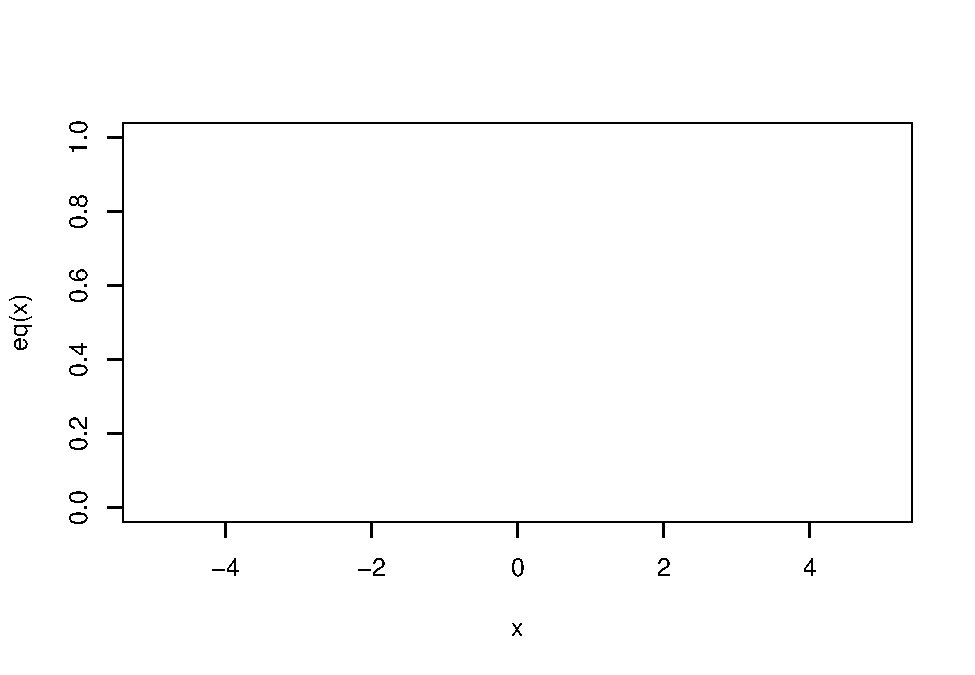
\includegraphics{ICC_project_files/figure-latex/unnamed-chunk-5-1.pdf}

\hypertarget{results}{%
\section{Results}\label{results}}

\hypertarget{discussion}{%
\section{Discussion}\label{discussion}}

\newpage

\hypertarget{references}{%
\section{References}\label{references}}

\begingroup
\setlength{\parindent}{-0.5in}
\setlength{\leftskip}{0.5in}

\hypertarget{refs}{}
\leavevmode\hypertarget{ref-R-markdown}{}%
Allaire, J., Horner, J., Xie, Y., Marti, V., \& Porte, N. (2019). \emph{Markdown: Render markdown with the c library 'sundown'}. Retrieved from \url{https://CRAN.R-project.org/package=markdown}

\leavevmode\hypertarget{ref-R-papaja}{}%
Aust, F., \& Barth, M. (2020). \emph{papaja: Create APA manuscripts with R Markdown}. Retrieved from \url{https://github.com/crsh/papaja}

\leavevmode\hypertarget{ref-R-shiny}{}%
Chang, W., Cheng, J., Allaire, J., Sievert, C., Schloerke, B., Xie, Y., \ldots{} Borges, B. (2021). \emph{Shiny: Web application framework for r}. Retrieved from \url{https://CRAN.R-project.org/package=shiny}

\leavevmode\hypertarget{ref-R-officer}{}%
Gohel, D. (2021). \emph{Officer: Manipulation of microsoft word and powerpoint documents}. Retrieved from \url{https://CRAN.R-project.org/package=officer}

\leavevmode\hypertarget{ref-R-purrr}{}%
Henry, L., \& Wickham, H. (2020). \emph{Purrr: Functional programming tools}. Retrieved from \url{https://CRAN.R-project.org/package=purrr}

\leavevmode\hypertarget{ref-kulas2017approximate}{}%
Kulas, J. T., Smith, J. A., \& Xu, H. (2017). Approximate functional relationship between irt and ctt item discrimination indices: A simulation, validation, and practical extension of lord's (1980) formula. \emph{Journal of Applied Measurement}, \emph{18}(4), 393--407.

\leavevmode\hypertarget{ref-R-tibble}{}%
Müller, K., \& Wickham, H. (2021). \emph{Tibble: Simple data frames}. Retrieved from \url{https://CRAN.R-project.org/package=tibble}

\leavevmode\hypertarget{ref-R-pdftools}{}%
Ooms, J. (2021). \emph{Pdftools: Text extraction, rendering and converting of pdf documents}. Retrieved from \url{https://CRAN.R-project.org/package=pdftools}

\leavevmode\hypertarget{ref-R-base}{}%
R Core Team. (2020). \emph{R: A language and environment for statistical computing}. Vienna, Austria: R Foundation for Statistical Computing. Retrieved from \url{https://www.R-project.org/}

\leavevmode\hypertarget{ref-R-formattable}{}%
Ren, K., \& Russell, K. (2021). \emph{Formattable: Create 'formattable' data structures}. Retrieved from \url{https://CRAN.R-project.org/package=formattable}

\leavevmode\hypertarget{ref-R-psych}{}%
Revelle, W. (2021). \emph{Psych: Procedures for psychological, psychometric, and personality research}. Evanston, Illinois: Northwestern University. Retrieved from \url{https://CRAN.R-project.org/package=psych}

\leavevmode\hypertarget{ref-R-jpeg}{}%
Urbanek, S. (2021). \emph{Jpeg: Read and write jpeg images}. Retrieved from \url{https://CRAN.R-project.org/package=jpeg}

\leavevmode\hypertarget{ref-R-reticulate}{}%
Ushey, K., Allaire, J., \& Tang, Y. (2021). \emph{Reticulate: Interface to 'python'}. Retrieved from \url{https://CRAN.R-project.org/package=reticulate}

\leavevmode\hypertarget{ref-R-ggplot2}{}%
Wickham, H. (2016). \emph{Ggplot2: Elegant graphics for data analysis}. Springer-Verlag New York. Retrieved from \url{https://ggplot2.tidyverse.org}

\leavevmode\hypertarget{ref-R-stringr}{}%
Wickham, H. (2019). \emph{Stringr: Simple, consistent wrappers for common string operations}. Retrieved from \url{https://CRAN.R-project.org/package=stringr}

\leavevmode\hypertarget{ref-R-forcats}{}%
Wickham, H. (2021a). \emph{Forcats: Tools for working with categorical variables (factors)}. Retrieved from \url{https://CRAN.R-project.org/package=forcats}

\leavevmode\hypertarget{ref-R-tidyr}{}%
Wickham, H. (2021b). \emph{Tidyr: Tidy messy data}. Retrieved from \url{https://CRAN.R-project.org/package=tidyr}

\leavevmode\hypertarget{ref-R-tidyverse}{}%
Wickham, H., Averick, M., Bryan, J., Chang, W., McGowan, L. D., François, R., \ldots{} Yutani, H. (2019). Welcome to the tidyverse. \emph{Journal of Open Source Software}, \emph{4}(43), 1686. \url{https://doi.org/10.21105/joss.01686}

\leavevmode\hypertarget{ref-R-readxl}{}%
Wickham, H., \& Bryan, J. (2019). \emph{Readxl: Read excel files}. Retrieved from \url{https://CRAN.R-project.org/package=readxl}

\leavevmode\hypertarget{ref-R-dplyr}{}%
Wickham, H., François, R., Henry, L., \& Müller, K. (2021). \emph{Dplyr: A grammar of data manipulation}. Retrieved from \url{https://CRAN.R-project.org/package=dplyr}

\leavevmode\hypertarget{ref-R-readr}{}%
Wickham, H., \& Hester, J. (2021). \emph{Readr: Read rectangular text data}. Retrieved from \url{https://CRAN.R-project.org/package=readr}

\leavevmode\hypertarget{ref-R-knitr}{}%
Xie, Y. (2015). \emph{Dynamic documents with R and knitr} (2nd ed.). Boca Raton, Florida: Chapman; Hall/CRC. Retrieved from \url{https://yihui.org/knitr/}

\leavevmode\hypertarget{ref-R-tinytex}{}%
Xie, Y. (2019). TinyTeX: A lightweight, cross-platform, and easy-to-maintain latex distribution based on tex live. \emph{TUGboat}, (1), 30--32. Retrieved from \url{http://tug.org/TUGboat/Contents/contents40-1.html}

\leavevmode\hypertarget{ref-R-rmarkdown_a}{}%
Xie, Y., Allaire, J. J., \& Grolemund, G. (2018). \emph{R markdown: The definitive guide}. Boca Raton, Florida: Chapman; Hall/CRC. Retrieved from \url{https://bookdown.org/yihui/rmarkdown}

\leavevmode\hypertarget{ref-R-DT}{}%
Xie, Y., Cheng, J., \& Tan, X. (2021). \emph{DT: A wrapper of the javascript library 'datatables'}. Retrieved from \url{https://CRAN.R-project.org/package=DT}

\leavevmode\hypertarget{ref-R-rmarkdown_b}{}%
Xie, Y., Dervieux, C., \& Riederer, E. (2020). \emph{R markdown cookbook}. Boca Raton, Florida: Chapman; Hall/CRC. Retrieved from \url{https://bookdown.org/yihui/rmarkdown-cookbook}

\endgroup


\end{document}
